%===============================================================================================================================
%================================================================= V I S T A S =================================================
%===============================================================================================================================
	\chapter{Vistas}
	\noindent En este apartado, se muestran las vistas finales de la aplicación web, mostrando cada uno de los módulos junto con su descripción y al actor que corresponde cada una de ellas.
		
		\begin{figure} [hbt!]
			\centering
			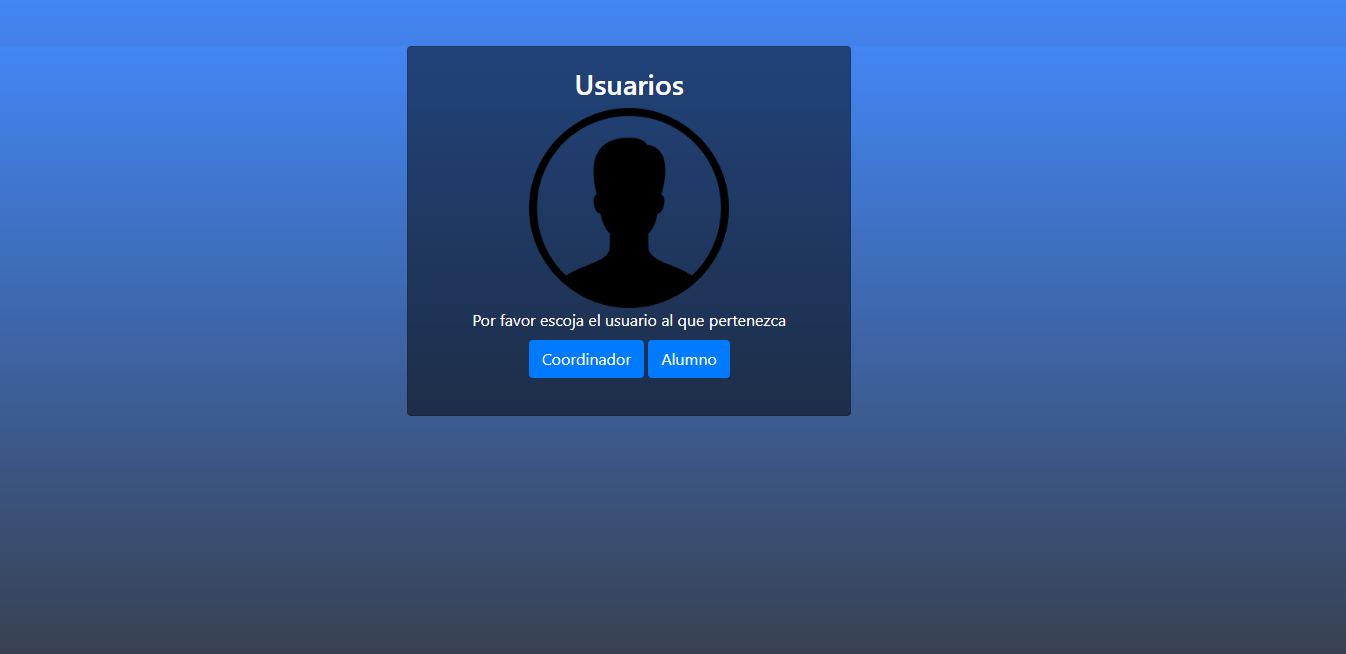
\includegraphics[width=10cm, height=6cm]{Imagenes/Vistas/VIsta1_TipoSesion}
			\caption{Vista que ayuda a definir el tipo de usuario que ingresará.}
			\label{VistaTipoSesion}
		\end{figure}
	
		\begin{figure} [hbt!]
			\centering
			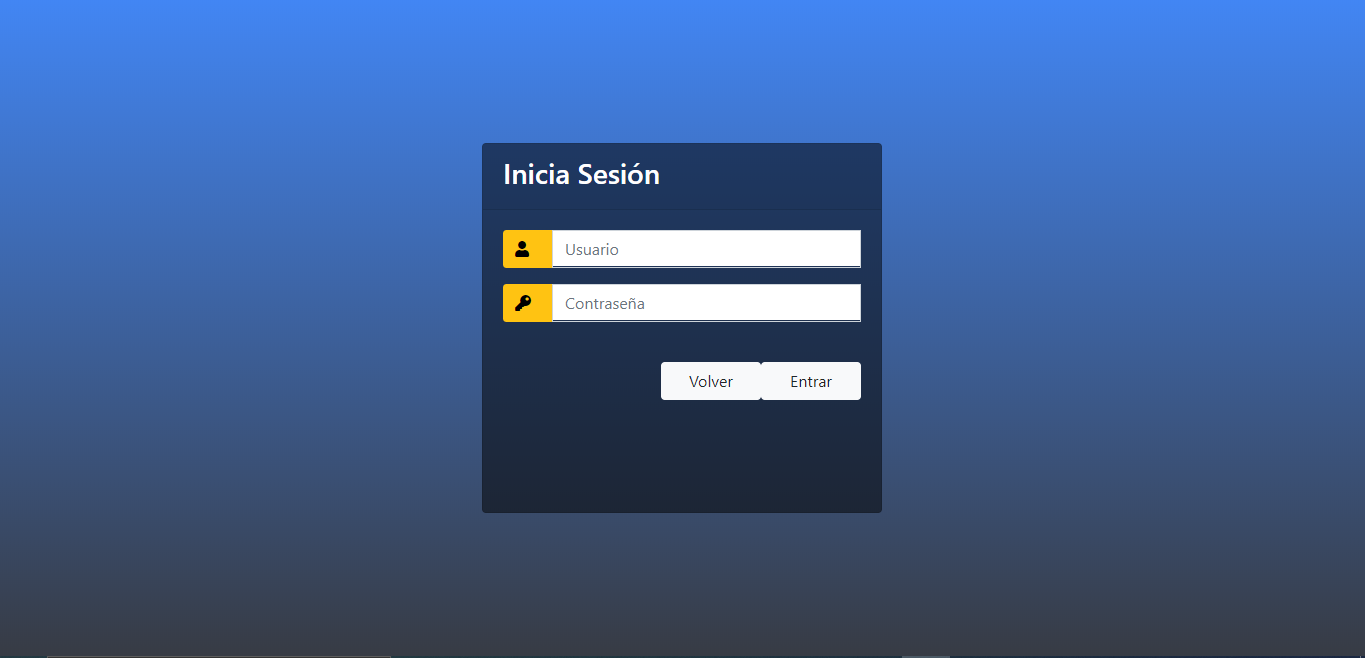
\includegraphics[width=10cm, height=6cm]{Imagenes/Vistas/Vista2_InicioSesionJFD}
			\caption{Vista del Inicio de Sesión para el Jefe de Fomento Deportivo y el Coordinador de una Unidad Académica.}
			\label{VistaInicioSesionJFD}
		\end{figure}
	
		\begin{figure} [hbt!]
			\centering
			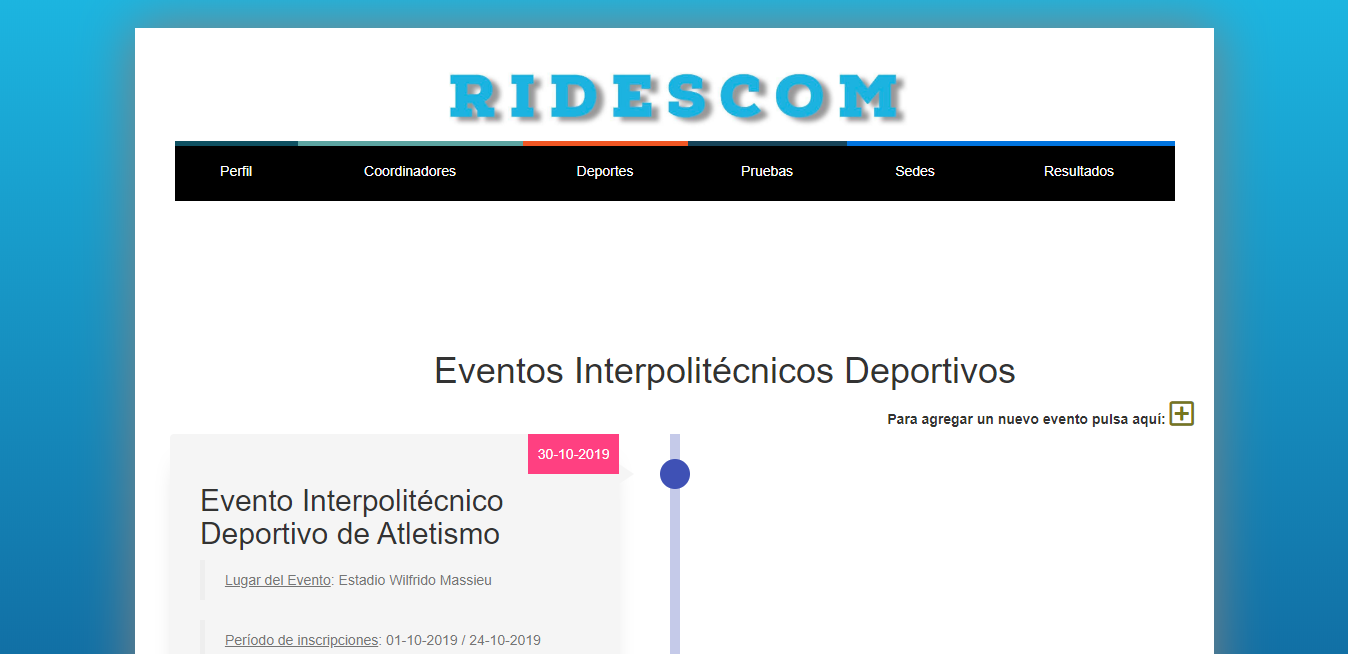
\includegraphics[width=10cm, height=6cm]{Imagenes/Vistas/Vista3_PrincipalJFD}
			\caption{Vista principal del Jefe de Fomento Deportivo (JFD).}
			\label{VistaPrincipalJFD}
		\end{figure}
			
		\begin{figure} [hbt!]
			\centering
			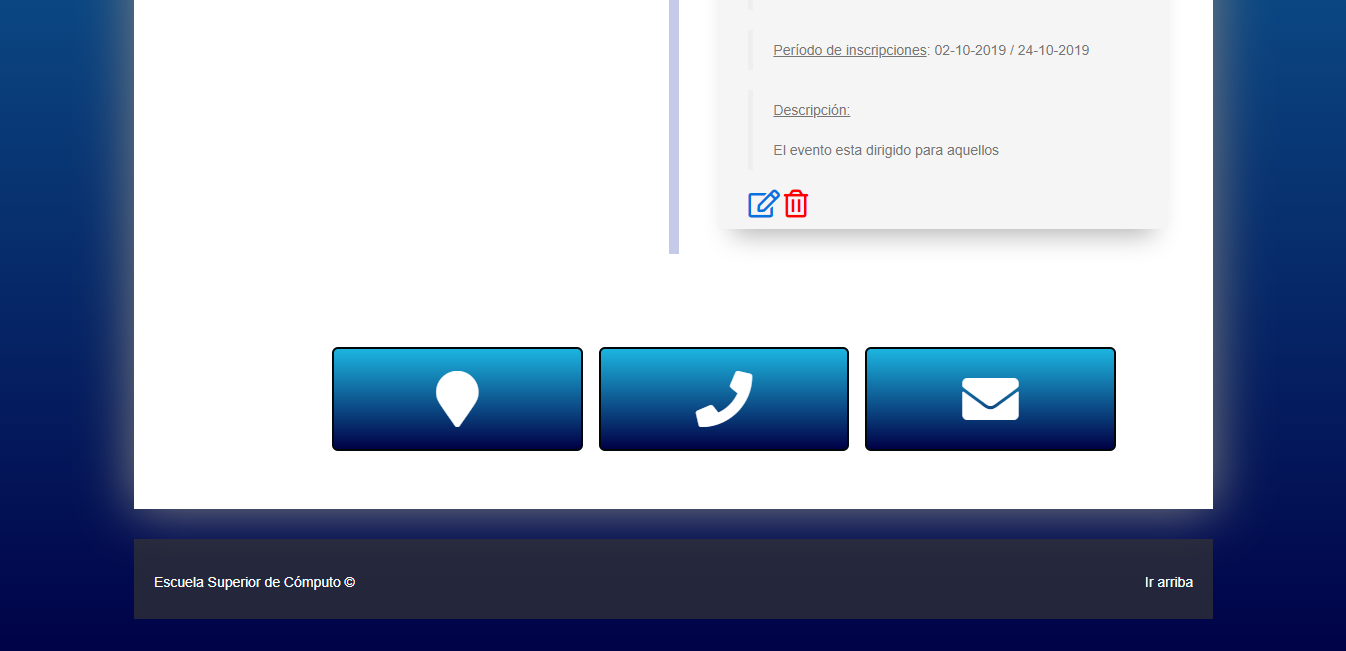
\includegraphics[width=10cm, height=6cm]{Imagenes/Vistas/Vista4_PrincipalJFD}
			\caption{Vista principal del Jefe de Fomento Deportivo continuación(JFD).}
			\label{VIstaPrincipalJFD1}
		\end{figure}
	
		\begin{figure} [hbt!]
			\centering
			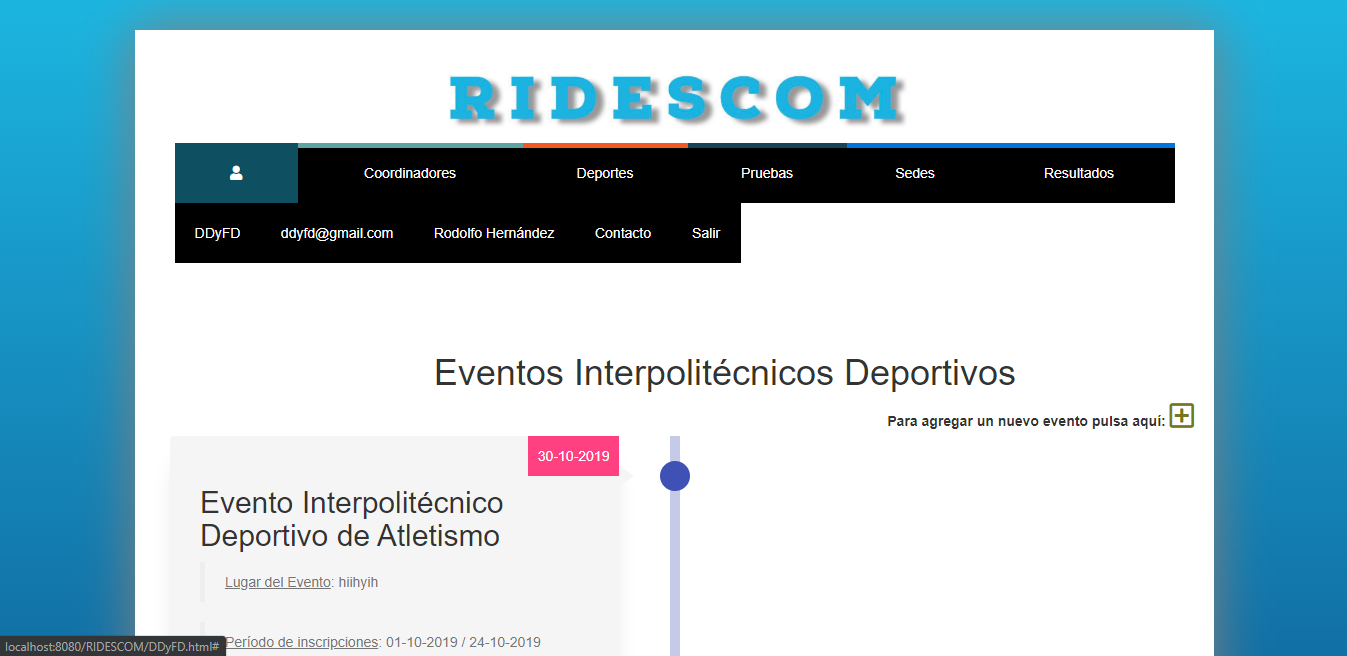
\includegraphics[width=10cm, height=6cm]{Imagenes/Vistas/Vista5_MenuUsuarioJFD}
			\caption{Vista que muestra datos del usuario en sesión.(Jefe de Fomento Deportivo)}
			\label{VistaMenuUsuario}
		\end{figure}
		
		\begin{figure} [hbt!]
			\centering
			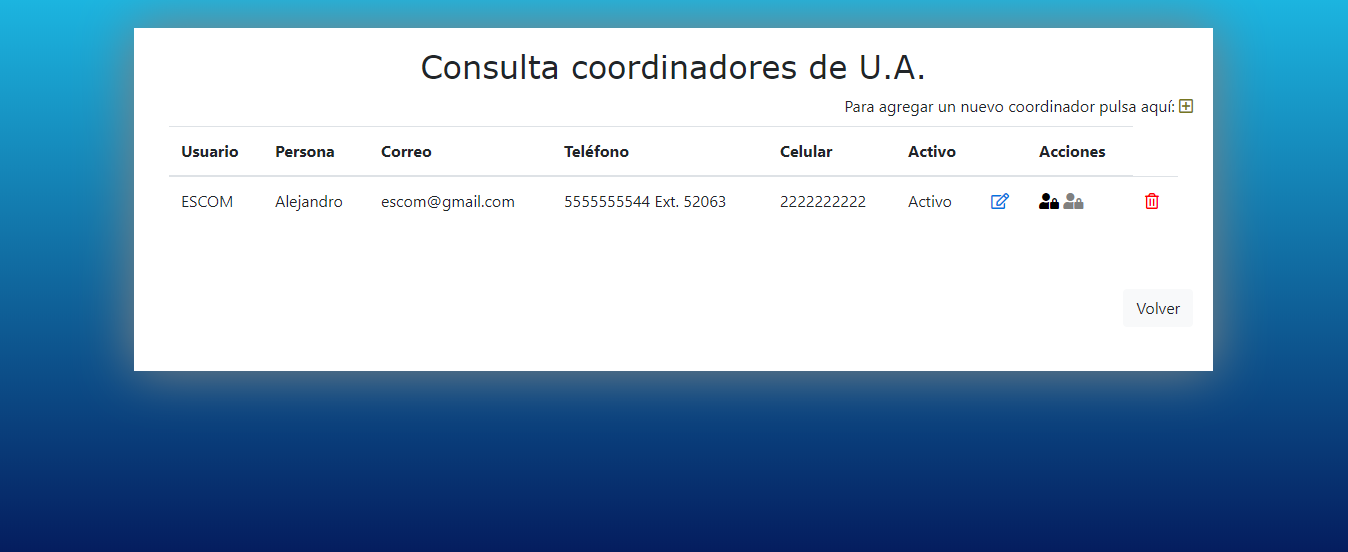
\includegraphics[width=10cm, height=6cm]{Imagenes/Vistas/Vista6_ConsultaCoordJFD}
			\caption{Vista donde se visualizan los Coordinadores de Unidades Académicas registrados.}
			\label{VistaConsultaCoord}
		\end{figure}
		
		\begin{figure} [hbt!]
			\centering
			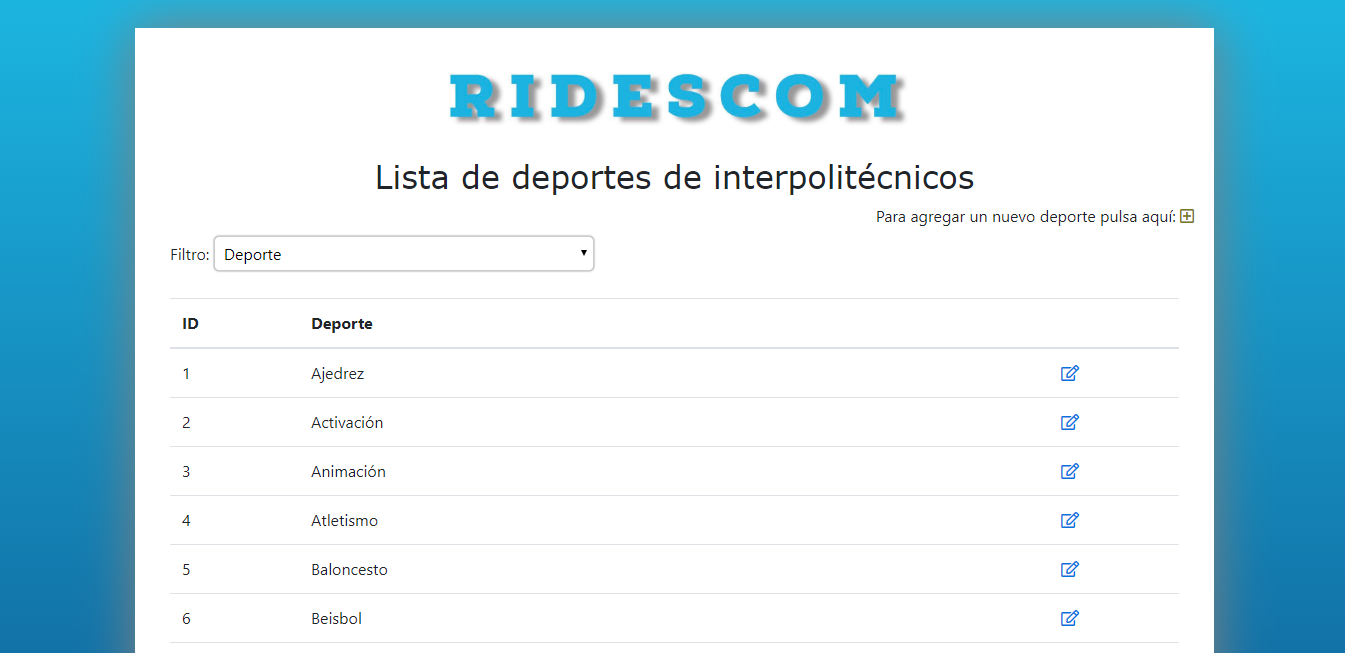
\includegraphics[width=10cm, height=6cm]{Imagenes/Vistas/Vista7_DeportesJFD}
			\caption{Vista en la que el Jefe de Fomento Deportivo visualiza los deportes que se practican actualmente en el Instituto Politécnico Nacional.}
			\label{VistaDeportes}
		\end{figure}
		
		\begin{figure} [hbt!]
			\centering
			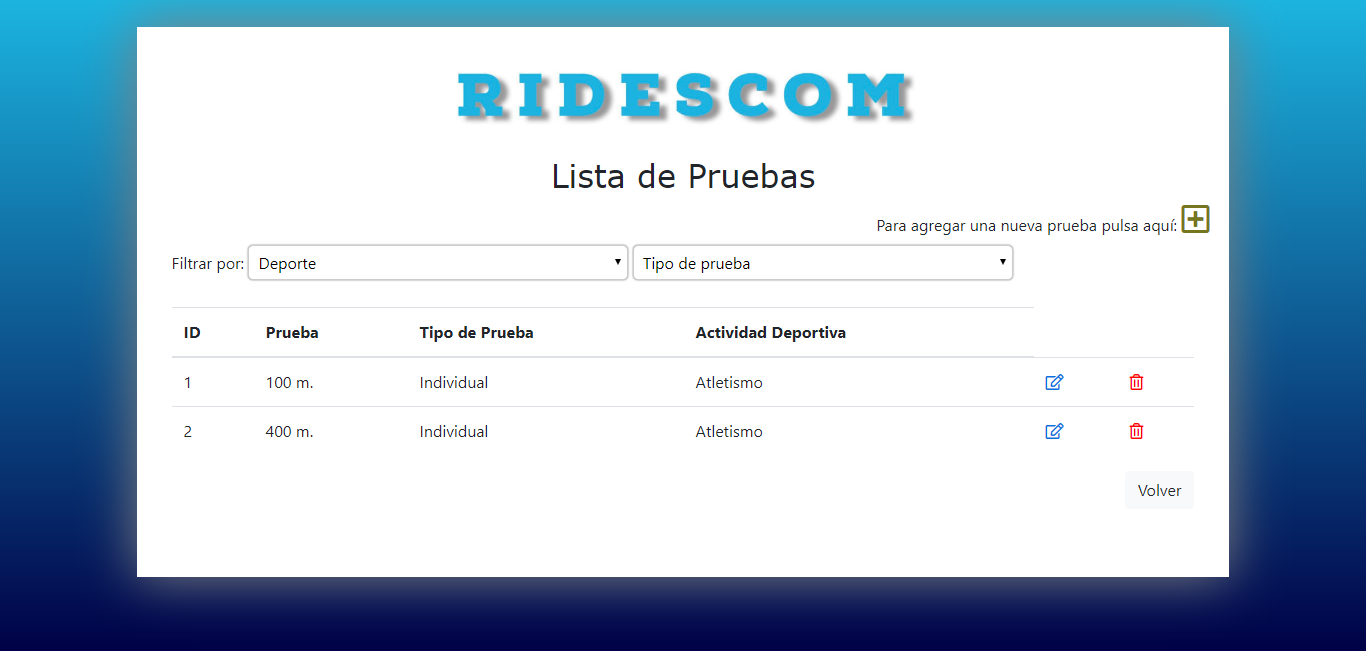
\includegraphics[width=10cm, height=6cm]{Imagenes/Vistas/Vista8_PruebaJFD}
			\caption{Vista donde el Jefe de Fomento Deportivo podrá ver las pruebas que han sido registradas.}
			\label{VistaPruebas}
		\end{figure}
	
		\begin{figure}
			\centering
			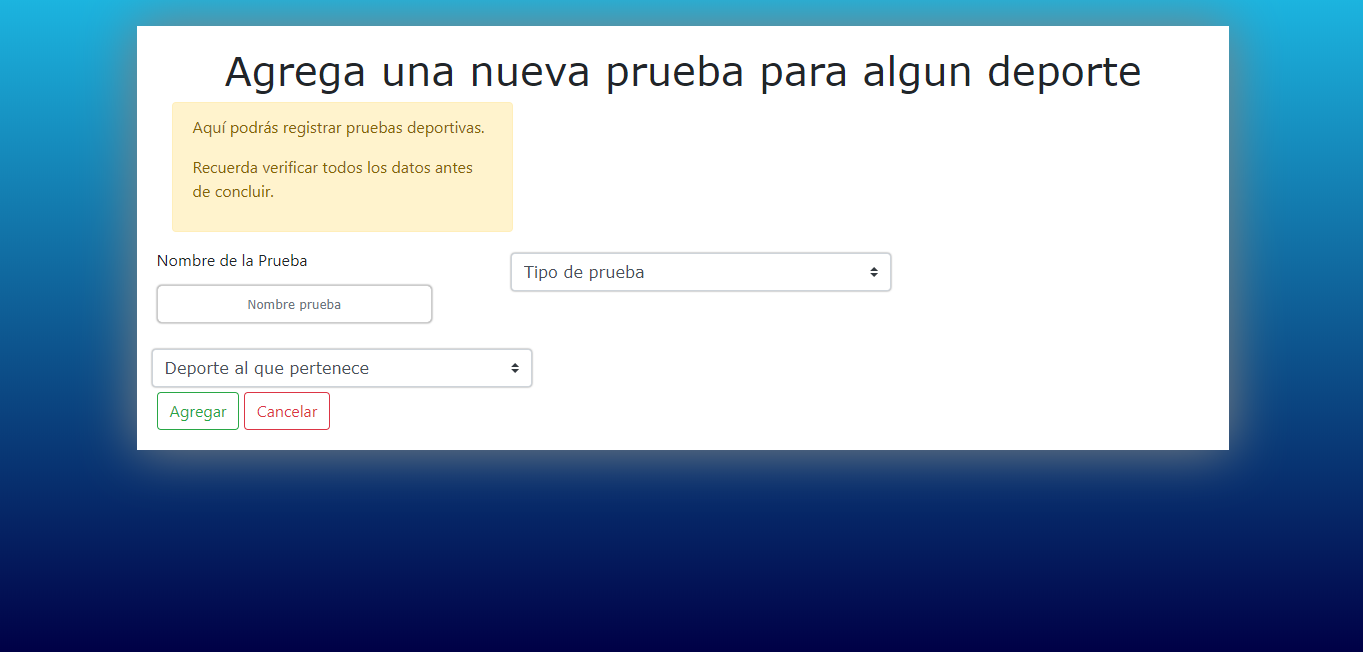
\includegraphics[width=10cm, height=6cm]{Imagenes/Vistas/Vista20_AgregaPrueba}
			\caption{Vista para agregar una prueba.}
			\label{VistaAgregaPrueba}
		\end{figure}
		
	
		\begin{figure} [hbt!]
			\centering
			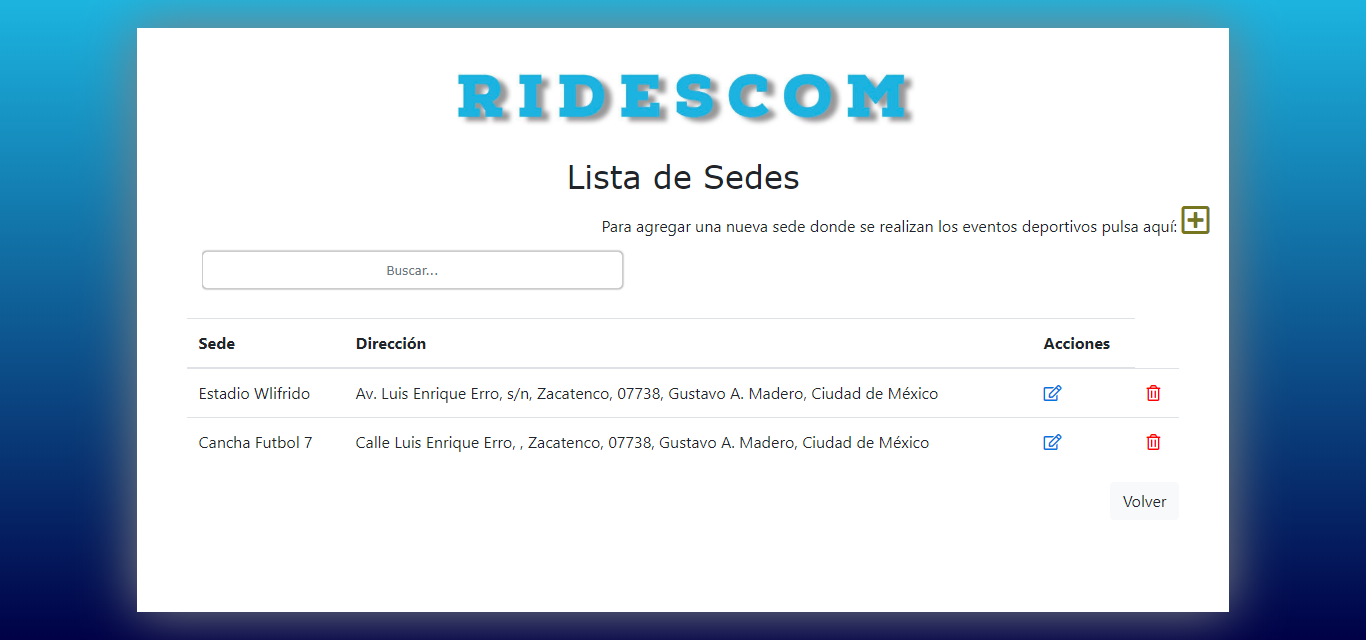
\includegraphics[width=10cm, height=6cm]{Imagenes/Vistas/Vista9_SedesJFD}
			\caption{Vista para visualizar las sedes donde se llevarán a cabo los eventos interpolitécnicos deportivos.}
			\label{VistaSedes}
		\end{figure}
		
		\begin{figure} [hbt!]
			\centering
			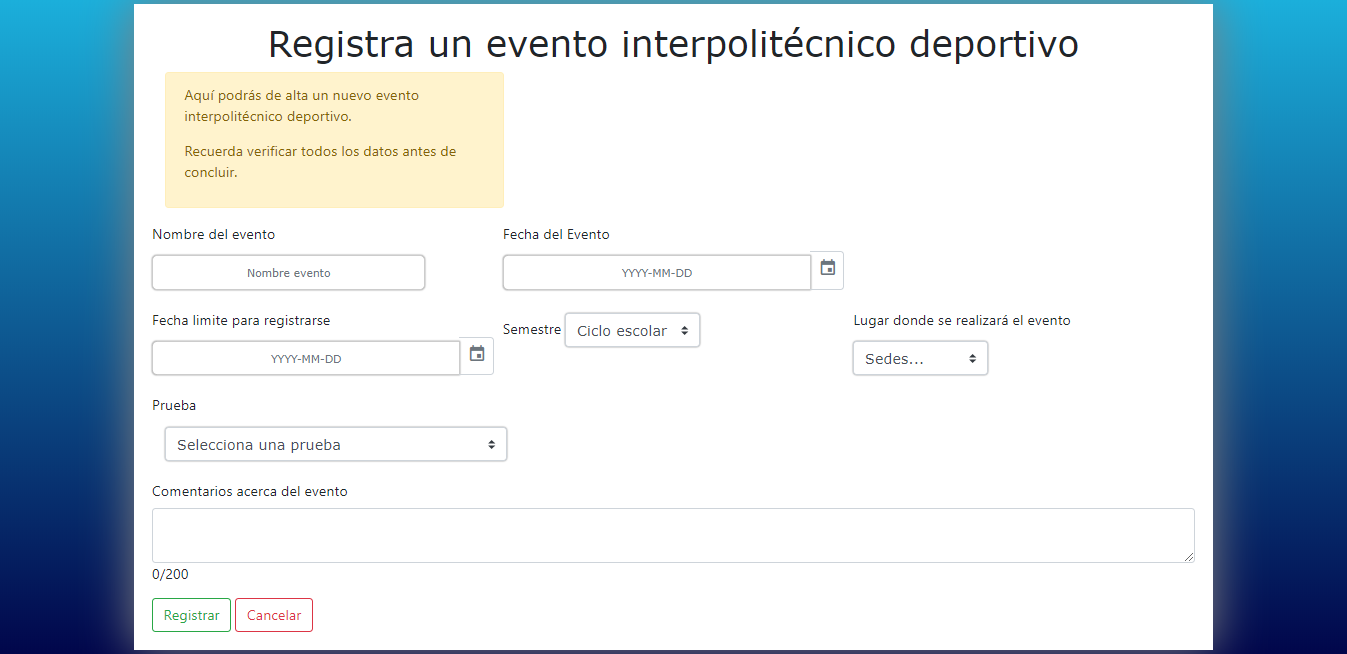
\includegraphics[width=10cm, height=6cm]{Imagenes/Vistas/Vista10_AgregaEvento}
			\caption{Vista en la que se puede agregar un Evento Interpolitécnico Deportivo.}
			\label{VistaAgregarEvento}
		\end{figure}
	
		\begin{figure} [hbt!]
			\centering
			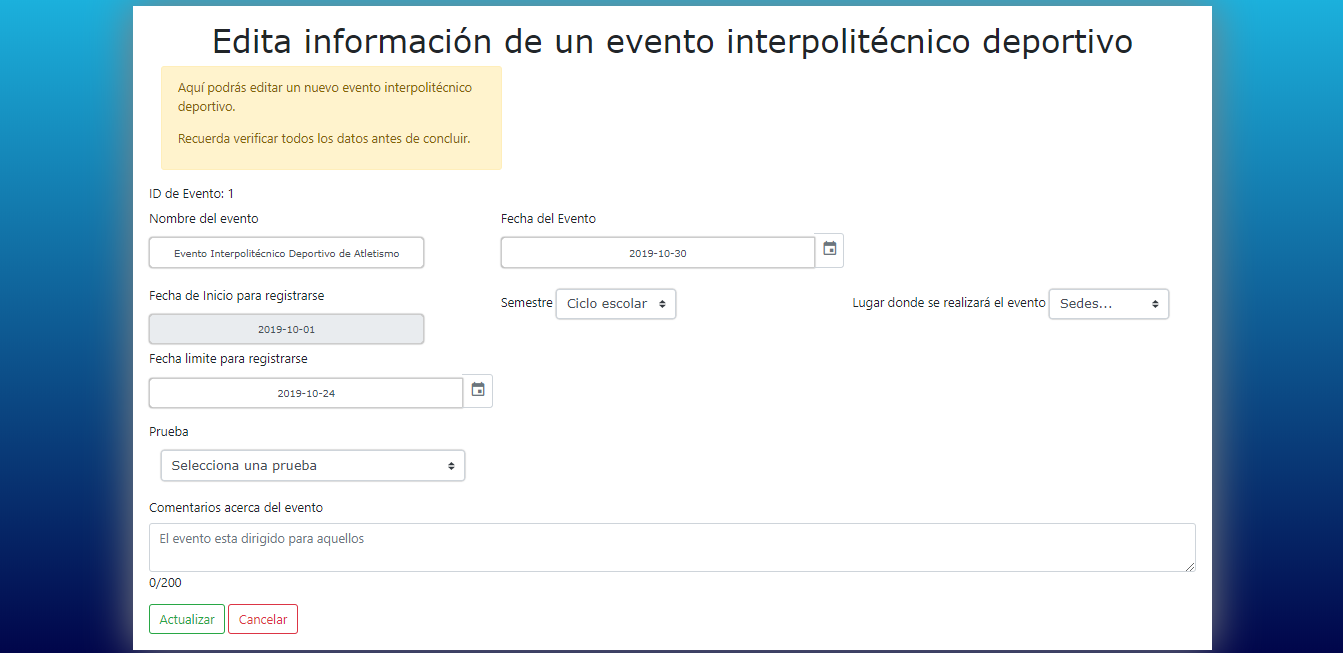
\includegraphics[width=10cm, height=6cm]{Imagenes/Vistas/Vista11_EditarEvento}
			\caption{Vista en la que se pueden editar los datos de un Evento Interpolitécnico Deportivo.}
			\label{VistaEditarEvento}
		\end{figure}
		
		\begin{figure} [hbt!]
			\centering
			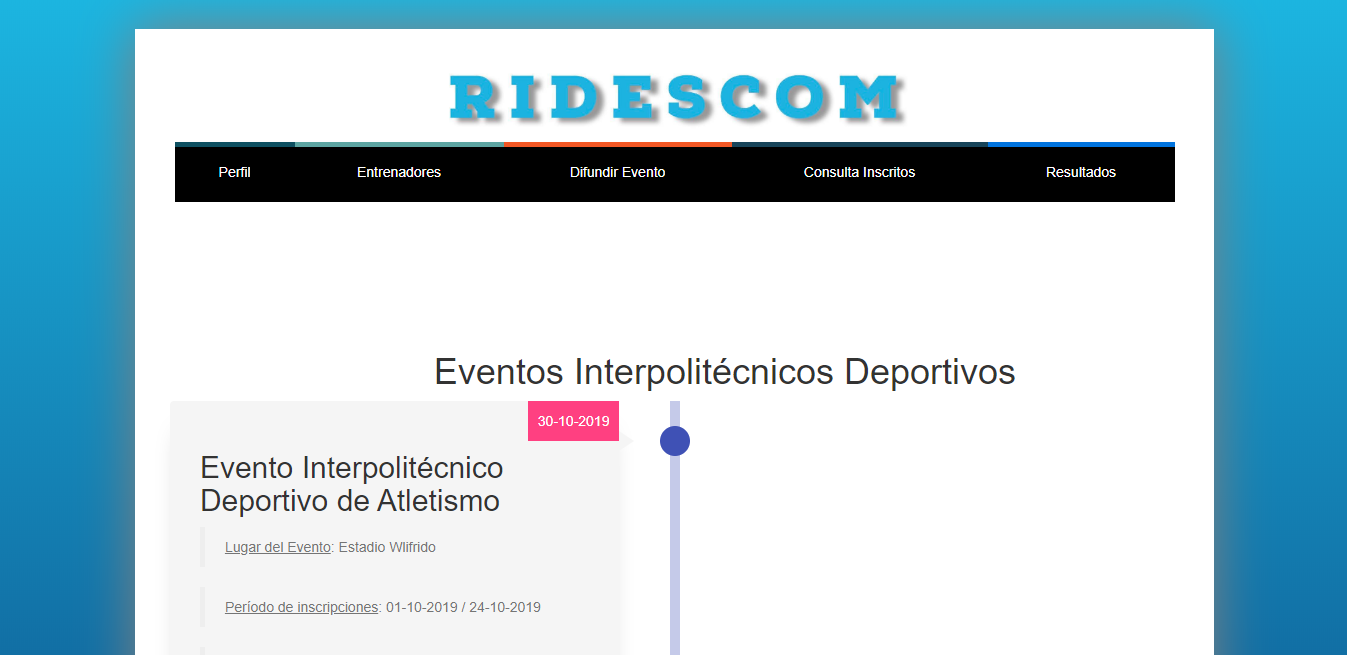
\includegraphics[width=10cm, height=6cm]{Imagenes/Vistas/Vista12_PrincipalCoord}
			\caption{Vista principal del Coordinador de la Unidad Académica.}
			\label{VistaPrincipalCoord}
		\end{figure}
		
		\begin{figure} [hbt!]
			\centering
			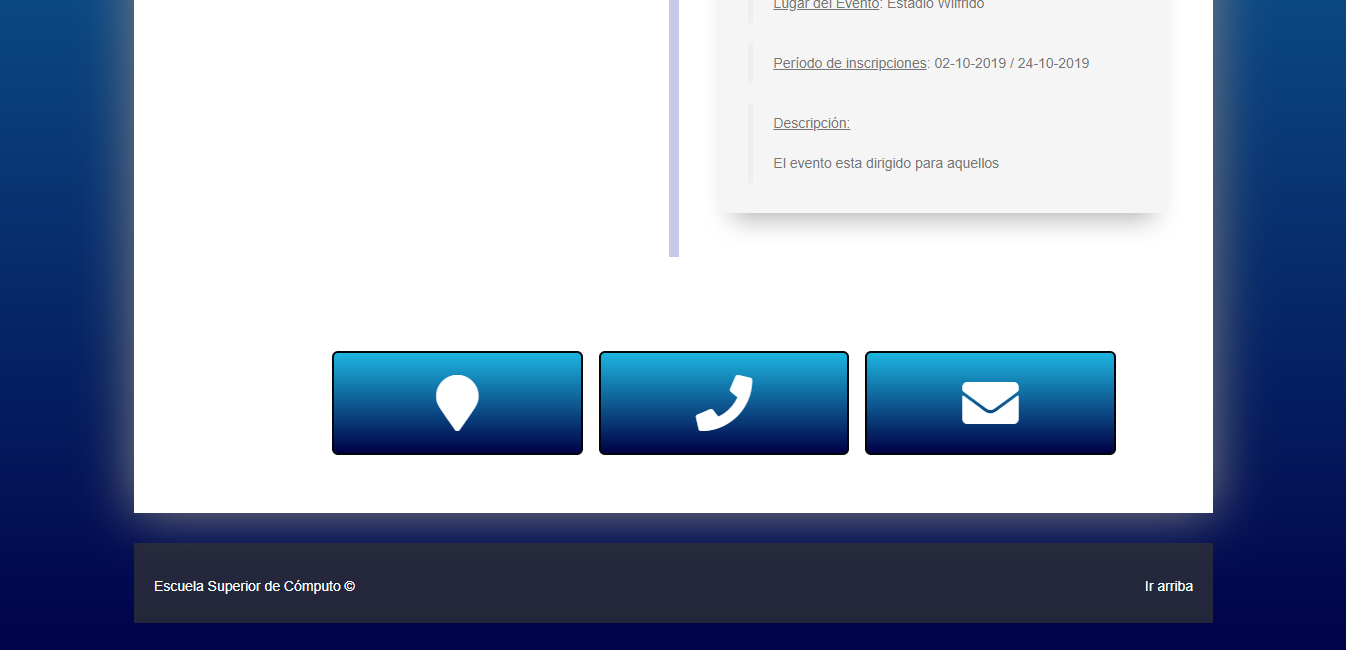
\includegraphics[width=10cm, height=6cm]{Imagenes/Vistas/Vista13_PrincipalCoord}
			\caption{Vistas principal del Coordinador de la Unidad Académica. (Continuación)}
			\label{VistaPrincipalCoord1}
		\end{figure}
		
		\begin{figure} [hbt!]
			\centering
			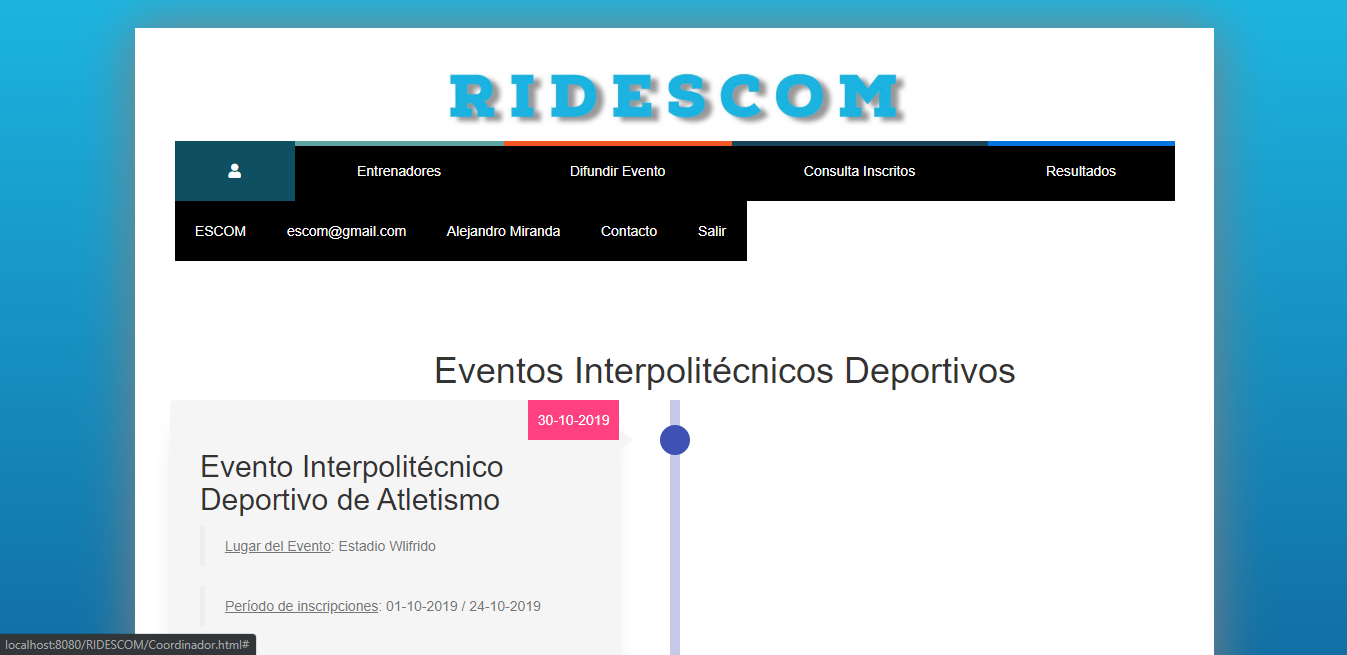
\includegraphics[width=10cm, height=6cm]{Imagenes/Vistas/Vista14_MenuUsuarioCoord}
			\caption{Vista que muestra datos del usuario en sesión.(Coordinador)}
			\label{VistaMenuCoord}
		\end{figure}
		
		\begin{figure} [hbt!]
			\centering
			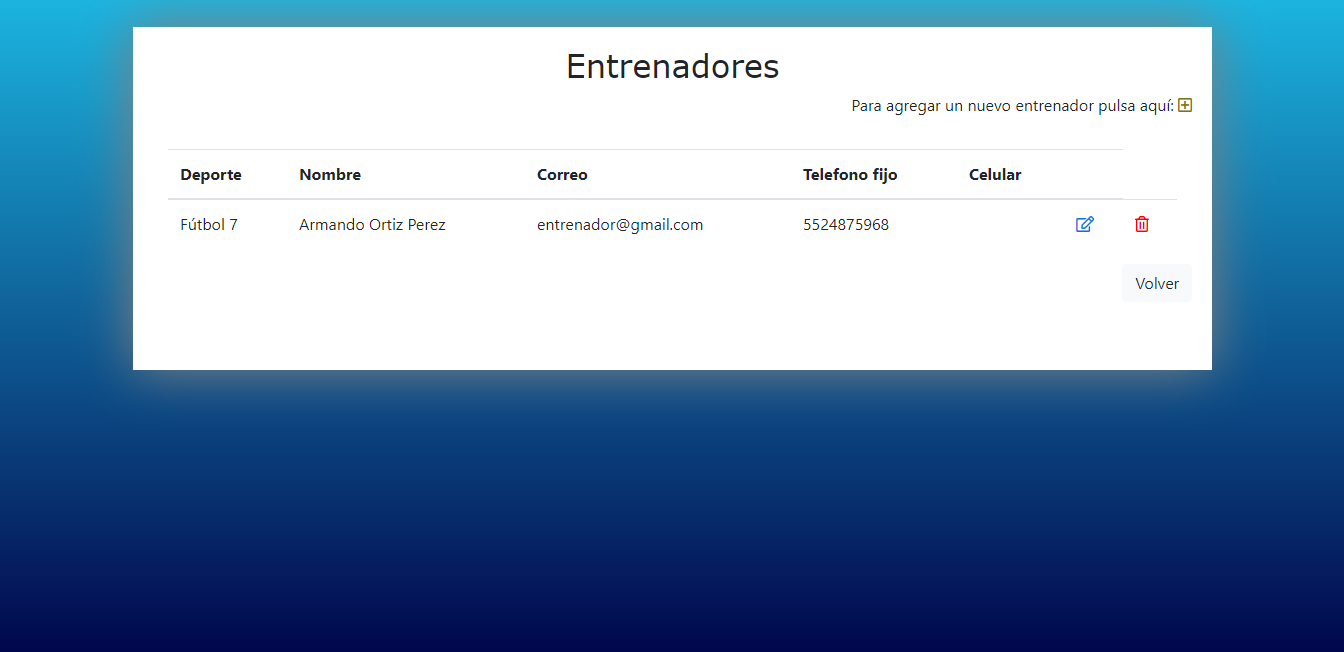
\includegraphics[width=10cm, height=6cm]{Imagenes/Vistas/Vista15_ConsultaEntrenador}
			\caption{Vista para la consulta de entrenadores.}
			\label{VistaConsultaEntrenador}
		\end{figure}
		
		\begin{figure} [hbt!]
			\centering
			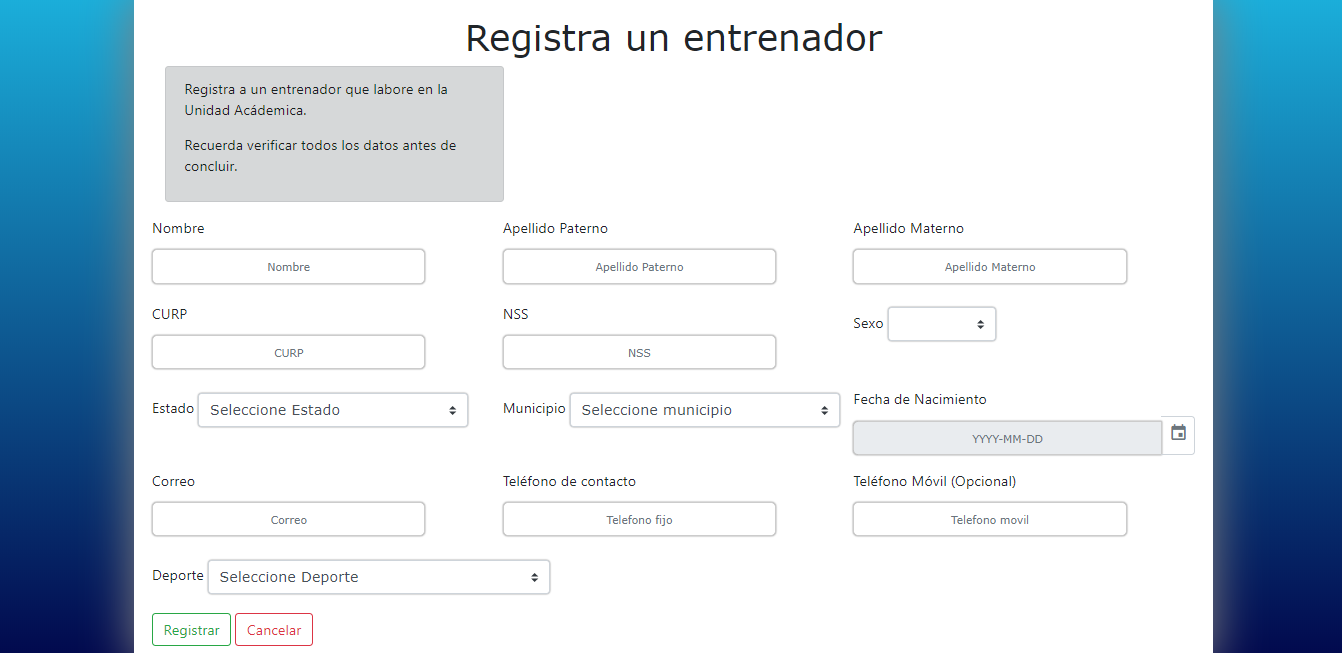
\includegraphics[width=10cm, height=6cm]{Imagenes/Vistas/Vista16_AgregaEntrenador}
			\caption{Vista para agregar a un entrenador.}
			\label{VistaAgregarEntrenador}
		\end{figure}
	
		\begin{figure} [hbt!]
			\centering
			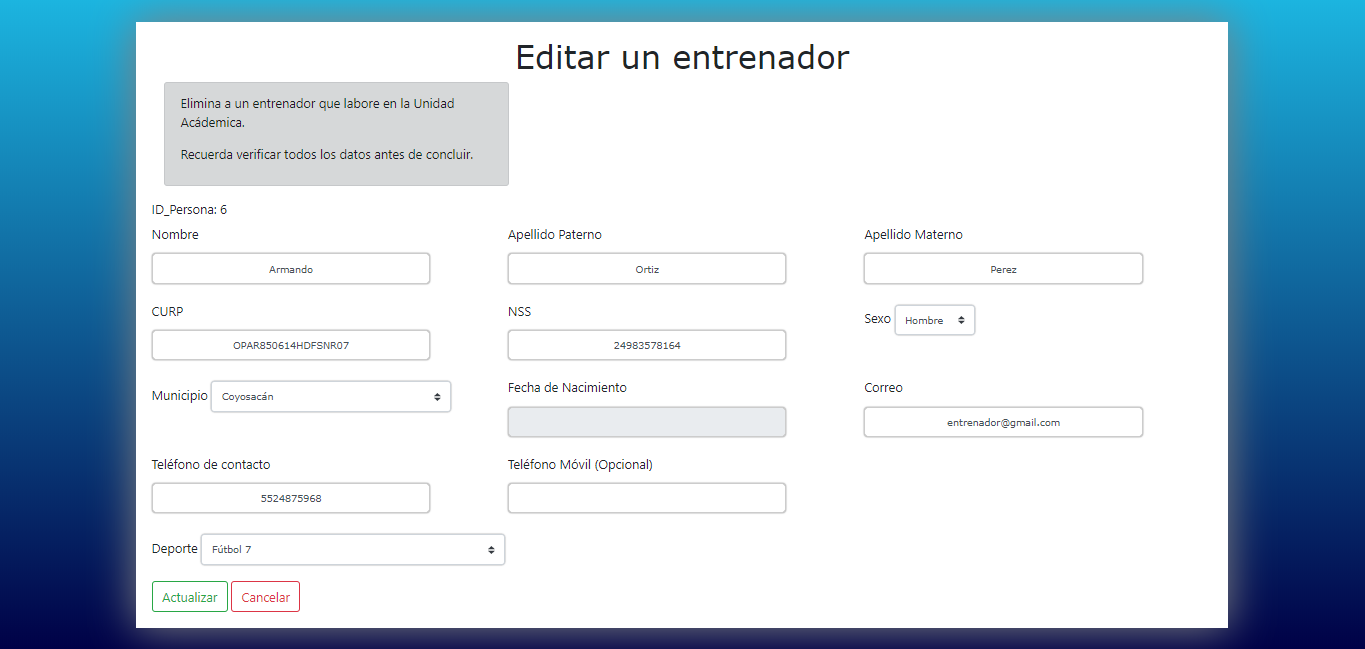
\includegraphics[width=10cm, height=6cm]{Imagenes/Vistas/Vista17_EditarEntrenador}
			\caption{Vista para editar los datos del entrenador.}
			\label{VistaEditarEntrenador}
		\end{figure}
		
		\begin{figure} [hbt!]
			\centering
			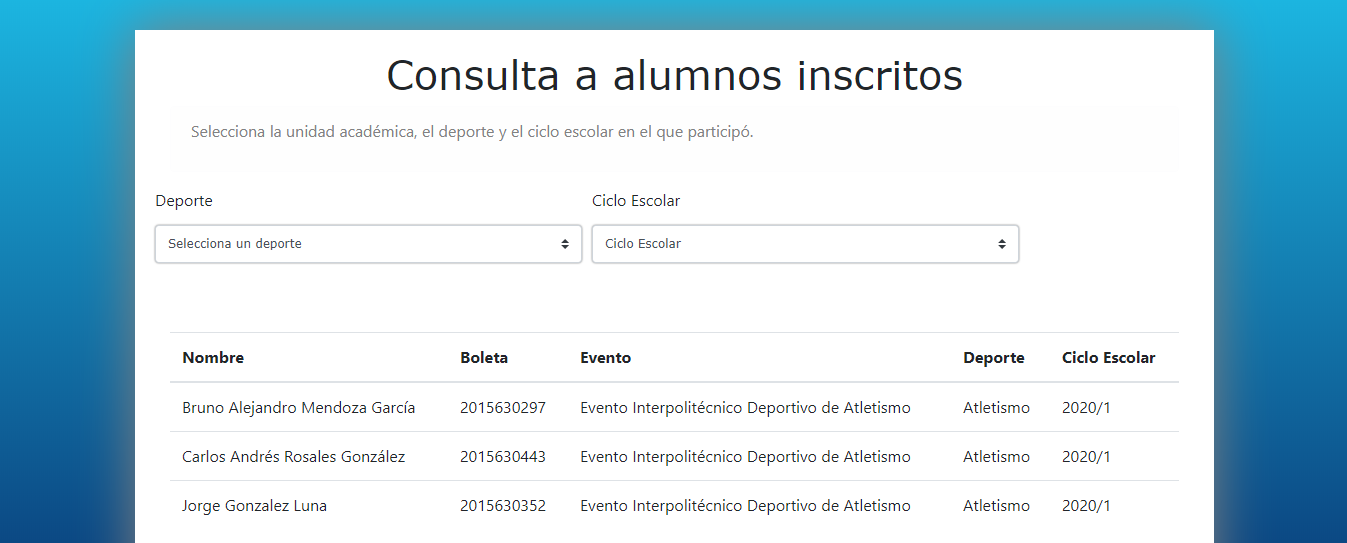
\includegraphics[width=10cm, height=6cm]{Imagenes/Vistas/Vista18_ConsultaInscritos}
			\caption{Vista para consultar los alumnos inscritos en algún Evento Interpolitécnico Deportivo.}
			\label{VistaConsultaInscritos}
		\end{figure}
		
		\begin{figure} [hbt!]
			\centering
			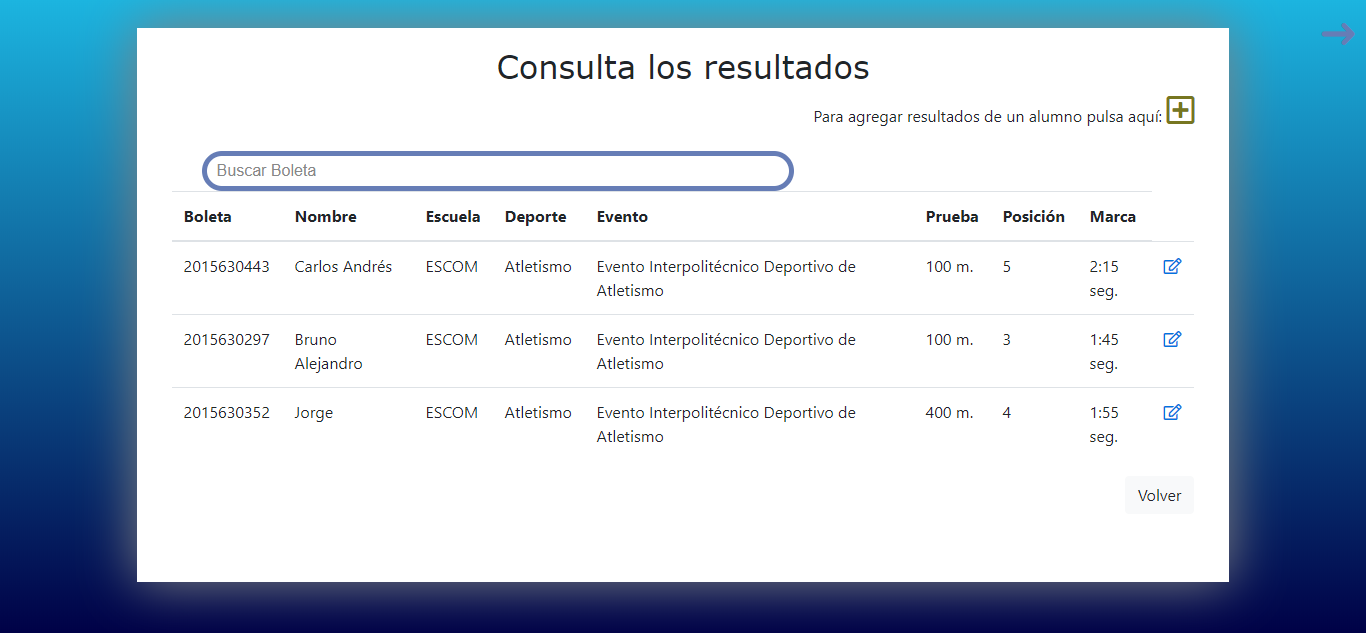
\includegraphics[width=10cm, height=6cm]{Imagenes/Vistas/Vista19_ConsultaResultados}
			\caption{Vista para consultar los resultados obtenidos por los participantes.}
			\label{VistaConsultaResultados}
		\end{figure}
		
		
